\usetikzlibrary{arrows.meta}
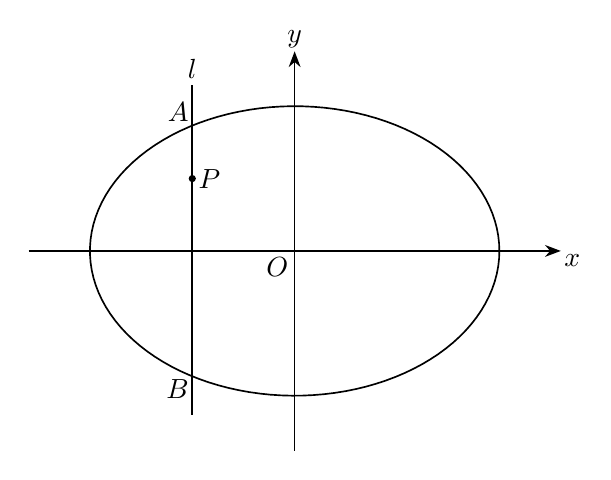
\begin{tikzpicture}[x=1.3cm,y=1.3cm,line width=.6pt,font=\normalsize,>=Stealth]
\coordinate (O) at (0,0);
\coordinate (A) at (-1,1.22474487);
\coordinate (B) at (-1,-1.22474487);
\coordinate (P) at (-1,0.70710678);
\draw plot[domain=0:360,samples=120] ({2*cos(\x)},{1.41421356*sin(\x)});
\draw (-1,-1.6)--(-1,1.62);
\draw[->] (-2.6,0)--(2.6,0) node[below right,inner sep=1pt] {$x$};
\draw[->] (0,-1.95)--(0,1.95) node[above,inner sep=1pt] {$y$};
\node[above,inner sep=2pt] at (-1,1.62) {$l$};
\fill (P) circle (1.3pt);
\node[above left,inner sep=1pt] at (A) {$A$};
\node[below left,inner sep=1pt] at (B) {$B$};
\node[right,inner sep=2pt] at (P) {$P$};
\node[below left,inner sep=2pt] at (O) {$O$};
\end{tikzpicture}
